\section{Linearni interpolacijski splajn}

Prilikom pokušaja interpolacije velikog broja točaka pojavljuje se problem sa oscilacijama na rubovima interpoliranih točaka gdje vrijedi:

$$
\lim_{n\to \infty}\max_{x\in[-1,1]}\left|f(x)-{\mathbf p}_n(x)\right| = +\infty
$$

Iz tog razloga se vrlo rijetko za interpolaciju koriste polinomi visokog stupnja ($>5$) jer ona ima loša svojstva.

Jedna od efikasnih metoda interpolacije je \textit{po dijelovima polinomna interpolacija} (engl. piecewise polynomial interpolation) gdje se na svim podsegmentima inicijalnog segmenta korise polinomi niskog stupnja:

$$
p_i \in \mathcal{P}_m
$$

gdje je $\mathcal{P}_m$ oznaka za \textbf{prsten polinoma} stupnja $m$.

Neka su zadani čvorovi interpolacije i \textbf{interpolicijski polinom dogovorenog i niskog stupnja} ($\phi$) na podsegmentima $[x_i,x_{i+1}]$ za $i\in[0,n\rangle$:

\begin{gather}
(x_i,y_i),\qquad i\in[0,n]\nonumber\\
\phi_{[x_i,x_{i+1}]} = p_i(x),\qquad i\in[0,n\rangle
\end{gather}

\begin{conditionbox}
    Iz uvijeta interpolacije $\phi(x_i) = y_i$ za $i\in[0,n]$:
    \begin{equation}
        \label{ls_continuation}
        p_{i-1}(x_i) = p_i(x_i)=y_i,\qquad i\in[1,n\rangle
    \end{equation}
    Dobivamo sljedećih $2n$ uvijeta kojima se osigurava neprekidnost funkcije $\phi(x)$:
    \begin{align}
        \label{ls_match_first}
        p_0(x_0) &= y_0\\
        \vdots\quad&\nonumber\\
        \label{ls_match_transition}
        p_{n-2}(x_{n-1}) &= p_{n-1}(x_n) = y_{n-1}\\
        \label{ls_match_last}
        p_{n-1}(x_n) &= y_n
    \end{align}
\end{conditionbox}

Uvijeti \ref{ls_continuation}, \ref{ls_match_first}, \ref{ls_match_transition} i \ref{ls_match_last} opisuju neprekidnost polinoma među interpoliranim podsegmentima.

Ako odaberemo da su polinomi $p_i(x)\in\mathcal{P}_1$ (polinomi prvog stupnja), tada imamo dovoljno uvjeta iz kojih možemo jedinstveno odrediti sve koeficijente linearnog interpolacijskog splajna.

\subsection{Linearni splajn}

Svakom podsegmentu $[x_i,x_{i+1}]$ pridužimo jedinstveni polinom $p_i(x)$ kojeg jednostavno zapisujemo u obliku lagrangeovog ili newtonovog interpolacijskog polinoma:

\begin{align*}
\text{Lagrangeov polinom:}\qquad p_i(x) =&\,\frac{x-x_{i+1}}{x_i-x_{i+1}}y_i + \frac{x-x_i}{x_{i+1}-x_i}y_{i+1}\\\\
\text{Newtonov polinom:}\qquad p_i(x) =&\,y_i + \frac{y_{i+1}-y_i}{x_{i+1}-x_i}(x-x_i)
\end{align*}

Linerani splajn se na kraju definira kao funkcija po dijelovima gdje je svaki dio definiran za pojedini segment kao pripadni polinom:

\begin{equation}
    \Phi(x)=\begin{cases}
        p_0(x),&x\in[x_0,x_1\rangle\\
        p_1(x),&x\in[x_1,x_2\rangle\\
        \quad\vdots&\\
        p_n(x),&x\in[x_n,x_{n+1}]\\
    \end{cases}
\end{equation}

\newpage

\begin{example}[određivanje linearnog splajna]
    Odredi linearni splajn ako su zadane sljedeće točke:

    \center
    \begin{tabular}{r|c|c|c|c|c}
        x&0&1&2&3&4\\
        \hline
        y&0&0&1&1&0
    \end{tabular}
\end{example}

\begin{multicols}{2}

Određujemo Newtonove interpolacijske polinome za sve tražene podsegmente:

\begin{align*}
    p_0(x)=y_0+\frac{y_1-y_0}{x_1-x_0}(x-x_0)&=0+\frac{0-0}{1-0}(x-0)=0\\
    p_1(x)=y_1+\frac{y_2-y_1}{x_2-x_1}(x-x_1)&=0+\frac{1-0}{2-1}(x-1)=x-1\\
    p_2(x)=y_2+\frac{y_3-y_2}{x_3-x_2}(x-x_2)&=1+\frac{1-1}{3-2}(x-2)=1\\
    p_3(x)=y_3+\frac{y_4-y_3}{x_4-x_3}(x-x_3)&=1+\frac{0-1}{4-3}(x-3)=4-x\\
\end{align*}

Te iz toga dobivamo formulu za linearni interpolacijski splajn:

$$
\Phi(x)=\begin{cases}
0,&x\in[0,1\rangle\\
x-1,&x\in[1,2\rangle\\
1,&x\in[2,3\rangle\\
4-x,&x\in[3,4]\\
\end{cases}
$$

\newcolumn

\begin{tikzpicture}
    \begin{axis}[
        domain=0:4,
        ymin=-1,ymax=2,
        ]
        \addplot[plotlinefound] expression[domain=0:1,samples=10]{0};
        \addplot[plotlinefound,color=cGreen] expression[domain=1:2,samples=10]{\x-1};
        \addplot[plotlinefound,color=cYellow] expression[domain=2:3,samples=10]{1};
        \addplot[plotlinefound,color=orange] expression[domain=3:4,samples=10]{4-\x};
        \addplot[plotinterpolated] coordinates {(0,0)};
        \addplot[plotinterpolated] coordinates {(1,0)};
        \addplot[plotinterpolated] coordinates {(2,1)};
        \addplot[plotinterpolated] coordinates {(3,1)};
        \addplot[plotinterpolated] coordinates {(4,0)};
    \end{axis}
\end{tikzpicture}

\end{multicols}

\subsection{Određivanje linearnog splajna u Pythonu}

\begin{example}
    Uporabom \codepkg{matplotlib} biblioteke, prikaži u Pythonu linearni splajn
    za podatke iz prethodnog primjera.
\end{example}

U sklopu \codepkg{numpy} biblioteke je sadržana \codefn{interp} funkcija koja
računa linearnu interpolaciju za \verb|xr| točke (prvi argument), pomoću ulaznih
\verb|x| vrijednosti (drugi argument) i njima sukladnih \verb|y| vrijednosti
(treći agrument).

\begin{multicols}{2}
    \input{../code/lin_spline.tex}

    \columnbreak

    \textbf{Rezultat prikaza}

    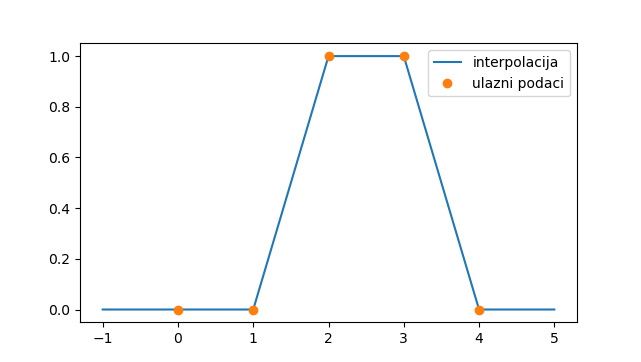
\includegraphics[width=\linewidth]{fig/lin_splajn.png}
\end{multicols}

Prethodno se koristila \codepkg{scipy.interpolate.}\codefn{interp1d} funkcija s argumentom \codenamedarg{kind}{\codestr{"linear"}}.

\newpage

\subsection{Ocjena greške}

Ocjena greške linearnog splajna slijedi iz ocjene greške interpolacijskog polinoma.

Neka je $f(x)\in\mathcal{C}^2[a,b]$. Tada je ocjena greške interpolacije funkcije $f$ linearnim splajnom:

$$
|f(x)-\phi(x)| \leq \frac{\omega(x)\max_{x\in[x_i,x_{i+1}]}|f''(x)|}{2!}
$$

Uvođenjem oznaka $h=\max_{i\in[1,n]}|x_i-x_{i-1}|$ i $M=\max_{x\in[a,b]}|f''(x)|$ tada je $\omega(x)\leq{h^2\over4}$ pa za ocjenu greške linearnim splajnom vrijedi:

$$
|f(x) - \phi(x)|\leq \frac{\text{M}h^2}{8}
$$

Odnosno možemo pisati:

\begin{equation*}
    f(x) = \phi(x) + \mathcal{O}(h^2),\qquad h\to0
\end{equation*}

Kako bi se postigla zadovoljavajuća točnost ovom interpolacijom je potreban veliki broj podsegmenata, no zbog jednostavnosti se ipak vrlo često koristi kod računalne grafike.

Kada je potrebno približno odrediti vrijednost $f(\xi), \xi\in[a,b]$, prvo je potrebno odrediti u kojem se intervalu nalazi $\xi$. Da bi odredili $i$ takav da je $x_i\leq\xi\leq x_{i+1}$ najčešće se koristi binarno pretraživanje koje koristi $\mathcal{O}(\log(n))$ operacija.

$$
f(\xi)\approx p_i(\xi)
$$

\newpage

\begin{example}[aproksimacija s točnošću]
    Aproksimirati funkciju $f(x) = \ln(x)$ na segmentu $[1,100]$ po dijelovima linearnom interpolacijom. Fiksirajmo traženu točnost $\varepsilon = 10^{-4}$ koju zahtijevamo na cijelom segmentu. Pronaći broj čvorova kako bi se postigla zadana točnost na:

    \begin{enumerate}
        \item ekvidistantnoj mreži s korakom $h$ na cijelom segmentu $[1,100]$
        \item podijeljenim podsegmentima $[1,2]$, $[2,7]$, $[7,100]$ gdje svaki od navedenih podsegmenata dijelimo ekvidistantnom mrežom čvorova s koracima $h_1$, $h_2$, $h_3$, respektivno.
    \end{enumerate}
\end{example}

\textbf{1)} Određujemo:
    $$
    f'(x) = {1\over x},\qquad f''(x)={1\over x^2}\text{, te}\qquad |f''(x)|=\left|{1\over x^2}\right|={1\over x^2}.
    $$
    Promatrana funkcija uvijek postiže svoj maksimum u lijevom kraju segmenta $[1,100]$.

Koristeći ocjenu greške za linearni splajn, dobivamo da je na segmentu $[1, 100]$
uz ekvidistantnu mrežu s korakom $h$ greška interpolacije

$$
|\Phi(x)-f(x)|\leq\frac{1\cdot h^2}{8}.
$$

U našem slučaju mora vrijediti $\displaystyle\frac{h^2}{8}\leq 10^{-4}$ što povlači $h\leq0.02828$.
S obzirom na to da je

$$
h=\frac{b-a}{n}=\frac{100-1}{n}=\frac{99}{n},
$$

dobivamo da je $n=3500.17$, a budući da je $n\in\mathbb{N}$, tada u formulu nije uključen posljednji rubni čvor, zaključujemo da nam je za zadanu točnost potrebno barem $3501+1=3502$ čvorova.

\bigskip

\textbf{2)} Na svakom zadanom podsegmentu greška interpolacije mora biti manja od $\varepsilon=10^{-4}$.

\begin{itemize}
    \item Za prvi podsegment $[1,2]$ vrijedi $\text{M}_2(f) = 1$ pa je $\frac{h_1^2}{8}\leq10^{-4}$ što povlači $h_1\leq0.02828$, a analognim postupkom kao u prethodnom slučaju dobivamo da je $n_1\geq35.35$, odnosno $n_1=36$.
    \item Na drugom podsegmentu $[2,7]$ vrijedi $\text{M}_2(f) = {1\over4}$ pa je ${1\over4}\cdot\frac{h_2^2}{8}\leq10^{-4}$ odnosno $h_2\leq0.05656$ pa je $n_2\geq88.38$, odnosno $n_2=89$.
    \item Na trećem podsegmentu $[7,100]$ vrijedi $\text{M}_2(f) = {1\over49}$ pa je ${1\over49}\cdot\frac{h_3^2}{8}\leq10^{-4}$ odnosno $h_3\leq0.19798$ pa je $n_3\geq469.73$, odnosno $n_3=470$.
\end{itemize}

\subsection{Nedostaci}

Dok je aproksimacija danih podataka linearnim splajnom može biti dovoljna u nekim slučajevima, prijelazi između segmenata mogu biti pre nagli i primjetni za druge primjene. Na primjer:

\begin{itemize}
    \item brzina kretanja tijela u prostoru se može doimati \textit{neprirodnom},
    \item razlike u brzini porasta/pada amplitude zvuka su osjetne, \dots
\end{itemize}
